\documentclass[12pt,a4paper]{article}

% ─── Codificación y fuentes ───────────────────────────────────────────────────
\usepackage[utf8]{inputenc}
\usepackage[T1]{fontenc}
\usepackage[spanish,es-nodecimaldot]{babel}
\usepackage{csquotes}   % requerido por biblatex con babel
\usepackage{lmodern}

% ─── Geometría y márgenes ────────────────────────────────────────────────────
\usepackage[
  top=2.5cm, bottom=2.5cm,
  left=3cm,  right=2.5cm,
  headheight=26pt
]{geometry}

% ─── Gráficos e imágenes ─────────────────────────────────────────────────────
\usepackage{graphicx}
\usepackage{float}
\graphicspath{{./}}

% ─── Color y diseño ──────────────────────────────────────────────────────────
\usepackage[dvipsnames,table]{xcolor}

% UTN institucional
\definecolor{utnazul}{RGB}{0,70,127}
\definecolor{utnceleste}{RGB}{0,153,204}
% Ariel brand  — Ocean Deep Blue / Sustainable Green / Tech Gold
\definecolor{arielblue}{RGB}{44,95,124}
\definecolor{arielgreen}{RGB}{64,145,108}
\definecolor{techgold}{RGB}{212,160,23}
% PesquerosEnIA brand — Marine Teal / Deep Ocean / Coral Warm
\definecolor{pescateal}{RGB}{5,150,105}
\definecolor{pescaocean}{RGB}{59,130,246}
\definecolor{coralwarm}{RGB}{249,115,22}
% Neutrales
\definecolor{stgray}{RGB}{90,90,90}
\definecolor{sandgray}{RGB}{120,113,108}

% ─── Tipografía de sección ───────────────────────────────────────────────────
\usepackage{titlesec}
\titleformat{\section}
  {\large\bfseries\color{utnazul}}
  {\thesection.}{0.8em}{}[\color{utnazul}\titlerule]
\titleformat{\subsection}
  {\normalsize\bfseries\color{arielblue}}
  {\thesubsection.}{0.6em}{}
\titleformat{\subsubsection}
  {\normalsize\bfseries\color{stgray}}
  {}{0em}{}

% ─── Encabezado y pie de página ──────────────────────────────────────────────
\usepackage{fancyhdr}
\pagestyle{fancy}
\fancyhf{}
\fancyhead[L]{%
  \raisebox{-3pt}{
\includegraphics[height=14pt]{logo_utn_frch_negro.png}}%
  \hspace{6pt}\small\color{stgray} UTN Facultad Regional Chubut}
\fancyhead[R]{%
  \small\color{stgray} Propuesta de Extensión 2026%
  \hspace{6pt}\raisebox{-3pt}{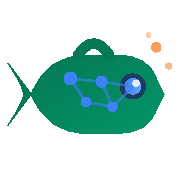
\includegraphics[height=14pt]{logo_pesqueros_symbol.pdf}}}
\fancyfoot[C]{\small\color{stgray}\thepage}
\renewcommand{\headrulewidth}{0.4pt}
\renewcommand{\headrule}{%
  \hbox to\headwidth{\color{utnazul}\leaders\hrule height\headrulewidth\hfill}}

% ─── Tablas ──────────────────────────────────────────────────────────────────
\usepackage{booktabs}
\usepackage{tabularx}
\usepackage{array}
\renewcommand{\arraystretch}{1.3}

% ─── Listas ──────────────────────────────────────────────────────────────────
\usepackage{enumitem}
\setlist[itemize]{leftmargin=1.5em, itemsep=2pt}
\setlist[enumerate]{leftmargin=1.5em, itemsep=2pt}

% ─── Cajas / recuadros ───────────────────────────────────────────────────────
\usepackage{caption}   % debe cargarse antes de tcolorbox/skins
\usepackage{tcolorbox}
\tcbuselibrary{skins,breakable}

% Caja para cada clase del programa
\newtcolorbox{clasebox}[2][]{
  enhanced,
  colback=utnazul!4,
  colframe=utnazul!50,
  fonttitle=\bfseries\small\color{white},
  coltitle=white,
  attach boxed title to top left={yshift=-2mm, xshift=4mm},
  boxed title style={colback=utnazul, colframe=utnazul},
  title={#2},
  left=6pt, right=6pt, top=10pt, bottom=6pt,
  #1
}

% Caja de datos de portada
\newtcolorbox{infobox}{
  enhanced,
  colback=utnceleste!8,
  colframe=utnceleste!50,
  boxrule=0.8pt,
  left=8pt, right=8pt, top=6pt, bottom=6pt
}

% Caja para cada docente (color como argumento)
\newtcolorbox{docentebox}[2][]{
  enhanced,
  colback=white,
  colframe=#1!60,
  coltitle=white,
  fonttitle=\bfseries\normalsize,
  attach boxed title to top left={yshift=-2mm, xshift=4mm},
  boxed title style={colback=#1, colframe=#1},
  title={#2},
  borderline west={3.5pt}{0pt}{#1},
  left=10pt, right=8pt, top=10pt, bottom=8pt,
  boxrule=0.4pt,
  breakable
}

% ─── Hipervínculos ───────────────────────────────────────────────────────────
\usepackage[
  colorlinks=true,
  linkcolor=utnazul,
  urlcolor=pescateal,
  citecolor=arielblue
]{hyperref}

% ─── Bibliografía ────────────────────────────────────────────────────────────
\usepackage[style=apa, backend=biber, sorting=nyt]{biblatex}
\addbibresource{referencias.bib}

% ─── Espaciado ───────────────────────────────────────────────────────────────
\usepackage{setspace}
\setstretch{1.15}
\setlength{\parskip}{6pt}
\setlength{\parindent}{0pt}

% ─────────────────────────────────────────────────────────────────────────────
\begin{document}
\pagenumbering{arabic}

% ═══════════════════════════════════════════════════════════════
%  PORTADA
% ═══════════════════════════════════════════════════════════════
\begin{titlepage}
  \centering
  \thispagestyle{empty}

  % ── Logos institucionales (UTN FRCh izq · PesquerosEnIA der) ─
  \noindent
  \begin{minipage}[c]{0.48\linewidth}
    \centering
    
\includegraphics[height=2.2cm]{logo_utn_frch_negro.png}
  \end{minipage}%
  \hfill
  \begin{minipage}[c]{0.48\linewidth}
    \centering
    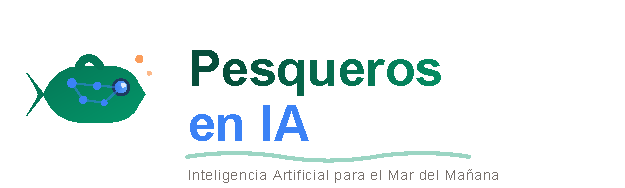
\includegraphics[height=1.9cm]{logo_pesqueros_full.pdf}
  \end{minipage}

  \vspace{0.4cm}
  \textcolor{utnazul}{\rule{\linewidth}{2pt}}\\[0.2cm]

  {\large\bfseries\color{utnazul}
    Universidad Tecnológica Nacional · Facultad Regional Chubut}\\[0.1cm]
  {\normalsize\color{stgray} Departamento de Ingeniería Pesquera}\\[0.05cm]
  {\small\color{utnceleste}
    \href{https://www.frch.utn.edu.ar}{www.frch.utn.edu.ar}}

  \vspace{0.5cm}
  \textcolor{utnazul}{\rule{\linewidth}{0.8pt}}\\[0.9cm]

  % ── Título ──────────────────────────────────────────────────
  {\fontsize{22}{28}\selectfont\bfseries\color{utnazul}
    Inteligencia Artificial}\\[0.2cm]
  {\fontsize{22}{28}\selectfont\bfseries\color{pescateal}
    Aplicada a la Producción Pesquera}\\[0.45cm]

  {\large\itshape\color{stgray}
    Propuesta de Curso de Extensión Universitaria}\\[0.25cm]
  {\normalsize\color{sandgray}
    \textit{``Inteligencia Artificial para el Mar del Mañana''} --- PesquerosEnIA}

  \vspace{0.6cm}

  % ── Ficha técnica ───────────────────────────────────────────
  \begin{infobox}
    \centering\small
    \begin{tabular}{ll@{\hspace{1.5cm}}ll}
      \textbf{Período}       & Ago 2026 -- May 2027 & \textbf{Modalidad}  & Híbrida \\
      \textbf{Localización}  & Puerto Madryn, Chubut & \textbf{Nivel}      & Básico--Intermedio \\
      \textbf{Dirección}     & Ing. Cristina Fernández & \textbf{Co-Dir.}  & Ing. S. Corvalán \\
      \textbf{Organiza}      & UTN Facultad Regional Chubut & \textbf{Comunidad} & PesquerosEnIA \\
    \end{tabular}
  \end{infobox}

  \vfill

  % ── Equipo docente ──────────────────────────────────────────
  {\normalsize\color{stgray}\textbf{Equipo docente}}\\[0.5cm]

  \begin{minipage}[t]{0.30\linewidth}\centering
    \textcolor{arielblue}{\rule{1.8cm}{1.5pt}}\\[4pt]
    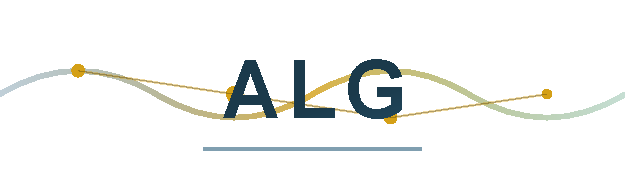
\includegraphics[height=0.65cm]{logo_ariel_symbol.pdf}\\[4pt]
    {\small\bfseries Ariel Luján Giamportone}\\
    {\footnotesize\color{stgray} Ing. Pesquero · Data Science · IA}
  \end{minipage}
  \hfill
  \begin{minipage}[t]{0.30\linewidth}\centering
    \textcolor{pescateal}{\rule{1.8cm}{1.5pt}}\\[4pt]
    \vspace{0.65cm}%
    {\small\bfseries Soraya Corvalán}\\
    {\footnotesize\color{stgray} Ing. Pesquera · Gestión · Sostenibilidad}
  \end{minipage}
  \hfill
  \begin{minipage}[t]{0.30\linewidth}\centering
    \textcolor{pescaocean}{\rule{1.8cm}{1.5pt}}\\[4pt]
    \vspace{0.65cm}%
    {\small\bfseries Damian Adolfo Giacone}\\
    {\footnotesize\color{stgray} Lic. Sistemas · Máster Ind. 4.0 · IA}
  \end{minipage}

  \vspace{0.55cm}
  \textcolor{utnazul}{\rule{\linewidth}{0.5pt}}\\[0.25cm]

  {\small\color{stgray}
    Material de acceso abierto bajo licencia \textbf{GPL-3.0}}\\
  {\small\color{pescateal}
    \url{https://github.com/PesquerosEnIA/curso-ia-produccion-pesquera}}

  \vspace{0.2cm}
  \textcolor{utnazul}{\rule{\linewidth}{2pt}}
\end{titlepage}

\tableofcontents
\newpage

% ═══════════════════════════════════════════════════════════════
%  1. RESUMEN EJECUTIVO
% ═══════════════════════════════════════════════════════════════
\section{Resumen Ejecutivo}

El presente documento constituye la propuesta académica del curso de extensión \textbf{``Inteligencia Artificial Aplicada a la Producción Pesquera''}, organizado por la Universidad Tecnológica Nacional, Facultad Regional Chubut (UTN FRCh), en colaboración con la comunidad \textbf{PesquerosEnIA}.

El curso tiene como propósito brindar a los profesionales del sector pesquero y acuícola argentino una formación aplicada en herramientas de inteligencia artificial, análisis de datos y automatización de procesos, orientada a las particularidades productivas, ambientales y regulatorias del sector.

La iniciativa se enmarca en un contexto de creciente digitalización de la industria pesquera global y responde a una demanda concreta de capacitación tecnológica en una región donde la pesca y la acuicultura constituyen pilares estratégicos de la economía patagónica.

% ═══════════════════════════════════════════════════════════════
%  2. FUNDAMENTACIÓN
% ═══════════════════════════════════════════════════════════════
\section{Fundamentación y Justificación}

\subsection{El sector pesquero argentino ante la transformación digital}

La Argentina posee una de las plataformas continentales más extensas del mundo, con una zona económica exclusiva (ZEE) de aproximadamente 1.000.000\,km², siendo el sector pesquero una fuente significativa de divisas y empleo en la región patagónica. Sin embargo, la adopción de tecnologías digitales en este sector ha sido históricamente más lenta que en otras industrias primarias como la agroindustria o la minería.

A nivel global, la Organización de las Naciones Unidas para la Alimentación y la Agricultura (FAO) ha señalado reiteradamente que la transformación digital ---y en particular la inteligencia artificial--- representa una oportunidad estratégica para mejorar la sostenibilidad, la trazabilidad y la eficiencia operativa de las pesquerías \parencite{FAO2022, FAO2024}. El concepto de \textit{Smart Fisheries} ---pesquerías inteligentes integradas por sensores, conectividad, datos y algoritmos de decisión--- es hoy una realidad en las principales flotas pesqueras del mundo y comienza a ganar terreno en América Latina.

\subsection{La inteligencia artificial como herramienta sectorial}

La IA no es una tecnología abstracta: sus aplicaciones concretas en el sector pesquero van desde la predicción de zonas de pesca mediante análisis de variables oceanográficas, hasta el control de calidad en planta por visión artificial, pasando por la optimización de rutas de flota y la automatización de informes regulatorios. Investigaciones recientes demuestran que el uso de modelos de aprendizaje automático puede reducir significativamente el esfuerzo de pesca y los costos operativos \parencite{Kroodsma2018}.

Iniciativas análogas en rubros afines demuestran la viabilidad y alta demanda de este tipo de formación para sectores productivos primarios en Argentina. El curso \textit{``IA Aplicada al Agro: Big Data, Automatización y Decisiones Inteligentes''} del Centro de Profesionales en Informática Aplicada (CPIA) constituye un antecedente directo de este modelo formativo \parencite{CPIA2026}. El sector pesquero, con sus particularidades de datos masivos ---oceanográficos, satelitales, de captura---, puede beneficiarse de una propuesta equivalente y adaptada a sus necesidades.

\subsection{La brecha de capacitación en el sector}

A pesar del potencial, existe una marcada brecha entre la disponibilidad de herramientas de IA y la capacidad de los profesionales del sector para utilizarlas. Los estudios de adopción tecnológica en industrias extractivas en América Latina señalan como principales barreras: la falta de formación específica, el escaso acceso a materiales en español adaptados al dominio, y la ausencia de comunidades de práctica que sostengan el aprendizaje \parencite{CEPAL2021, BID2020}.

Este curso aborda directamente esa brecha, ofreciendo formación práctica, contextualizada y en idioma español, respaldada por una comunidad de profesionales del propio sector.

% ═══════════════════════════════════════════════════════════════
%  3. ANTECEDENTES
% ═══════════════════════════════════════════════════════════════
\section{Antecedentes y Experiencia Acumulada}

\subsection{I CONIPE 2019 --- Minicurso ``Industria 4.0: ¿es posible?''}

En el marco del \textbf{I Congreso Nacional de Ingeniería Pesquera (CONIPE 2019)}, celebrado en la UTN FRCh los días 29 y 30 de noviembre de 2019, el equipo dictó el minicurso \textbf{``Industria 4.0: ¿es posible?: el desafío de la adopción de la tecnología en el proceso productivo pesquero''} con una carga de 8 horas \parencite{Giacone2019}.

\textbf{Docentes:} Giacone, D.; Corvalán, S.; González, C.

Este minicurso constituyó uno de los primeros antecedentes sistemáticos de formación en transformación digital dirigida específicamente a profesionales del sector pesquero argentino en el ámbito de la UTN, abordando la brecha tecnológica y las condiciones de adopción de la Industria 4.0 en el proceso productivo pesquero.

\subsection{I CONIPE 2019 --- Mesa redonda ``Industria 4.0 en el sector pesquero''}

En el mismo evento se coordinó la mesa redonda \textbf{``Industria 4.0 en el sector pesquero: la nueva revolución digital''}, con participación interdisciplinaria de referentes académicos y profesionales del sector \parencite{Corvalan2019}.

\textbf{Coordinadora:} Corvalán, S.\\
\textbf{Ponentes:} Dra.\ Zanfrillo, A.; Lic.\ Giacone, D.; Ing.\ Fábrega, A.; Ing.\ Giamportone, A.\,L.

La presentación se encuentra publicada en el Anuario de Jornadas, Encuentros y Actividades de la UTN (AJEA):
\begin{center}
  \url{https://rtyc.utn.edu.ar/index.php/ajea/article/view/873/792}
\end{center}

\subsection{CONIPE 2025 --- Puerto Madryn}

En el marco del \textbf{Congreso Nacional de Ingeniería Pesquera (CONIPE 2025)}, celebrado en Puerto Madryn, la comunidad PesquerosEnIA impartió el curso \textbf{``Alfabetización en Ciencia de Datos e Inteligencia Artificial para Profesionales del Sector Pesquero y Acuícola''} \parencite{PesquerosEnIA2025}. Estructurado en 8 módulos, cubrió desde fundamentos de Python y manipulación de datos hasta introducción a modelos de machine learning aplicados a pesquerías.

La experiencia permitió validar la demanda de capacitación en el sector y ajustar los contenidos a las necesidades reales de los participantes, sentando las bases metodológicas y didácticas del presente curso. Material disponible en acceso abierto:
\begin{center}
  \url{https://github.com/PesquerosEnIA/curso_alfabetizacion_CONIPE25}
\end{center}

\subsection{ML \& Deep Learning for Fisheries Engineers (PesquerosEnIA)}

La comunidad PesquerosEnIA publica en acceso abierto el compendio \textbf{``Machine Learning and Deep Learning for Fisheries Engineers''} \parencite{PesquerosEnIAML2024}, una colección de notebooks Jupyter con aplicaciones de ML/DL contextualizadas al sector pesquero argentino: predicción de zonas de pesca, estimación de abundancia de especies, clasificación automática por visión artificial y optimización de operaciones de flota.

\subsection{Trabajos previos del equipo docente}

Los integrantes del equipo docente acumulan experiencia concreta en el desarrollo de modelos computacionales aplicados al sector:

\begin{itemize}
  \item \textbf{Modelo hidrodinámico para redes de acuicultura:} modelo predictivo de fuerzas hidrodinámicas sobre estructuras de cultivo, con variables ambientales reales.\\
        \url{https://github.com/arielgiamportone/Hydrodinamic_model_Aquaculture_nets}

  \item \textbf{Modelo de red de arrastre en el canal Beagle:} análisis de selectividad y optimización de artes de pesca para especies del Atlántico Sur.\\
        \url{https://github.com/arielgiamportone/Trawl_net_model_in_Advanced_Excel}

  \item \textbf{Selectividad de artes de pesca:} análisis estadístico avanzado (MLE) de selectividad para gestión pesquera sostenible.\\
        \url{https://github.com/arielgiamportone/Selectividad_artes_de_pesca}

  \item \textbf{Machine Learning para planificación y operaciones:} aplicación de ML en planificación operativa, adaptable a gestión de flotas y campañas pesqueras.\\
        \url{https://github.com/arielgiamportone/Machine_Learning_for_Sales_and_operations_Planning}
\end{itemize}

% ═══════════════════════════════════════════════════════════════
%  4. OBJETIVOS
% ═══════════════════════════════════════════════════════════════
\section{Objetivos}

\subsection{Objetivo General}

Brindar a los profesionales del sector pesquero y acuícola argentino una formación práctica en inteligencia artificial y análisis de datos, orientada a mejorar la eficiencia operativa, la sostenibilidad y la toma de decisiones basada en evidencia en sus ámbitos de trabajo.

\subsection{Objetivos Específicos}

\begin{enumerate}
  \item Comprender el panorama actual de la transformación digital en el sector pesquero global y argentino, identificando oportunidades y barreras de adopción.
  \item Dominar el uso de modelos de lenguaje (LLMs) y técnicas de \textit{prompting} para automatizar tareas operativas y de análisis en el sector.
  \item Identificar, acceder y explorar las principales fuentes de datos del dominio pesquero: oceanográficos, satelitales, AIS/VMS, registros de captura y datos de planta.
  \item Aplicar conceptos de machine learning para construir modelos predictivos de zonas de pesca, abundancia de especies y patrones de captura.
  \item Reconocer las aplicaciones de visión artificial para control de calidad, clasificación de especies y automatización en plantas procesadoras.
  \item Utilizar herramientas de optimización e inteligencia artificial para mejorar la eficiencia de flotas pesqueras y la planificación de campañas.
  \item Construir tableros de visualización y análisis de datos para la toma de decisiones estratégicas y operativas en el sector.
\end{enumerate}

% ═══════════════════════════════════════════════════════════════
%  5. DESTINATARIOS
% ═══════════════════════════════════════════════════════════════
\section{Destinatarios}

El curso está dirigido a:

\begin{itemize}
  \item \textbf{Ingenieros pesqueros y acuícolas} --- con interés en incorporar herramientas digitales a su práctica profesional.
  \item \textbf{Biólogos marinos y oceanógrafos} --- que trabajen con datos de poblaciones, ecosistemas o monitoreo ambiental.
  \item \textbf{Técnicos y operadores} --- de barcos pesqueros, plantas procesadoras y centros de acuicultura.
  \item \textbf{Investigadores y docentes} --- vinculados a INIDEP, CONICET y universidades nacionales.
  \item \textbf{Profesionales de gestión y regulación} --- de organismos como la Subsecretaría de Pesca y Acuicultura, SENASA o entes provinciales.
\end{itemize}

\textbf{Perfil de ingreso:} No se requiere experiencia previa en programación ni en inteligencia artificial. Se recomienda familiaridad básica con herramientas informáticas y lectura comprensiva en inglés técnico básico.

% ═══════════════════════════════════════════════════════════════
%  6. PROGRAMA
% ═══════════════════════════════════════════════════════════════
\section{Programa de Contenidos}

El curso se organiza en \textbf{10 unidades}, con los contenidos mínimos aprobados por el Consejo Federal Pesquero, en modalidad híbrida (Agosto 2026 -- Mayo 2027).

\begin{clasebox}{Clase 1 — Estrategia y Transformación Digital en el Sector Pesquero}
  \textit{Docentes: Ariel Giamportone · Soraya Corvalán · María Ana Reussi · Soledad Gurisich}\\[4pt]
  Panorama de la transformación digital global y en el sector pesquero argentino. Concepto de \textit{Smart Fisheries}. Casos de uso de IA en barcos pesqueros, monitoreo del mar y plantas de procesamiento. Desafíos del sector: sostenibilidad, eficiencia de flotas, trazabilidad y control de calidad.
\end{clasebox}

\begin{clasebox}{Clase 2 — Fundamentos de IA y Modelos de Lenguaje (LLMs)}
  \textit{Docente: Damian Adolfo Giacone}\\[4pt]
  Diferencia entre IA tradicional y generativa. Funcionamiento conceptual de los modelos generativos. Aplicaciones en el sector: análisis de reportes de captura, generación de informes técnicos, asistencia para cumplimiento normativo. Limitaciones y uso responsable.
\end{clasebox}

\begin{clasebox}{Clase 3 — Prompting y Diseño de Asistentes de IA}
  \textit{Docente: Damian Adolfo Giacone}\\[4pt]
  Concepto de \textit{prompt} como interfaz. Técnicas: prompt directo, con contexto, iterativo, CAR (Contexto--Acción--Rol), \textit{Chain of Thought} y \textit{Few-Shot Prompting}. Diseño de asistentes para análisis de capturas, normativa pesquera y reportes de producción.
\end{clasebox}

\begin{clasebox}{Clase 4 — Datos y Sensores del Dominio Pesquero}
  \textit{Docentes: Ariel Giamportone · Soraya Corvalán}\\[4pt]
  Fuentes de datos en la actividad pesquera: oceanográficos, satelitales, AIS/VMS, GPS y registros de captura. Variables ambientales clave: temperatura superficial del mar (SST), corrientes, profundidad y clorofila. Plataformas de datos abiertos: INIDEP, Copernicus, NOAA y Global Fishing Watch. Ejercicio práctico con dataset oceanográfico real.
\end{clasebox}

\begin{clasebox}{Clase 5 — Arquitectura de Datos y Big Data en Pesca}
  \textit{Docente: Damian Adolfo Giacone}\\[4pt]
  Arquitecturas de datos para el sector pesquero: integración de sensores, plataformas en la nube y procesamiento masivo. Aplicación de modelos analíticos para predicción de zonas de pesca y monitoreo de operaciones.
\end{clasebox}

\begin{clasebox}{Clase 6 — Machine Learning y Modelos Predictivos en Pesca}
  \textit{Docentes: Damian Adolfo Giacone · Ariel Giamportone}\\[4pt]
  Aprendizaje automático aplicado a la actividad pesquera. Modelos predictivos para identificar zonas de pesca, estimar abundancia de especies y analizar patrones de captura. Evaluación con métricas relevantes para el sector. Ejercicio práctico con datos reales.
\end{clasebox}

\begin{clasebox}{Clase 7 — Visión Artificial en Plantas Pesqueras}
  \textit{Docentes: Damian Adolfo Giacone · Soraya Corvalán · Dr. Juan D. González · Martín I. Errázquin}\\[4pt]
  Visión por computadora y análisis de imágenes. Aplicaciones: clasificación automática de especies, conteo de peces, medición de talla y detección de defectos en plantas procesadoras. Integración de sistemas de visión artificial en líneas de producción.
\end{clasebox}

\begin{clasebox}{Clase 8 — Optimización de Operaciones y Agentes de IA}
  \textit{Docentes: Damian Adolfo Giacone · Ariel Giamportone}\\[4pt]
  Optimización de rutas de barcos, reducción del consumo de combustible y planificación de campañas pesqueras. Mantenimiento predictivo de embarcaciones. Agentes de IA para monitoreo autónomo de flotas y plantas.
\end{clasebox}

\begin{clasebox}{Clase 9 — Visualización y Dashboards para la Toma de Decisiones}
  \textit{Docente: Damian Adolfo Giacone}\\[4pt]
  De datos pesqueros a información accionable. \textit{Dashboards} para monitoreo de capturas, rendimiento de flotas y eficiencia de procesamiento. Herramientas: Excel avanzado, Tableau y Power BI. Trazabilidad digital del producto.
\end{clasebox}

\begin{clasebox}{Clase 10 — Cierre, Conclusiones y Hoja de Ruta}
  \textit{Docentes: Soraya Corvalán · Ariel Giamportone}\\[4pt]
  Síntesis del recorrido: de los datos a las decisiones en el sector pesquero. Hoja de ruta personal para continuar aprendiendo IA en el sector. Presentación de recursos abiertos de la comunidad PesquerosEnIA y próximos espacios de colaboración.
\end{clasebox}

% ═══════════════════════════════════════════════════════════════
%  7. METODOLOGÍA
% ═══════════════════════════════════════════════════════════════
\section{Metodología}

El curso adopta un enfoque de \textbf{aprendizaje basado en problemas del dominio} (\textit{problem-based learning}):

\begin{itemize}
  \item Clases sincrónicas de 2 horas: exposición teórica (40\,\%) y ejercicios prácticos (60\,\%).
  \item Notebooks Jupyter interactivos disponibles en repositorio público, ejecutables sin instalación mediante Google Colab.
  \item Datasets reales y abiertos del sector: INIDEP, Copernicus Marine Service, NOAA, Global Fishing Watch.
  \item Ejemplos contextualizados al sector pesquero argentino en todos los módulos.
  \item Material completamente en español. Repositorio público bajo licencia GPL-3.0.
\end{itemize}

\begin{table}[H]
  \centering
  \caption{Herramientas y plataformas del curso}
  \begin{tabular}{@{}ll@{}}
    \toprule
    \textbf{Herramienta} & \textbf{Uso} \\
    \midrule
    Google Colab / Jupyter & Ejecución de notebooks Python \\
    Python (pandas, scikit-learn, matplotlib) & Análisis y modelado de datos \\
    Power BI / Tableau / Excel & Visualización y dashboards \\
    GitHub & Repositorio de materiales \\
    Plataforma de videoconferencia & Clases sincrónicas \\
    \bottomrule
  \end{tabular}
\end{table}

% ═══════════════════════════════════════════════════════════════
%  8. EVALUACIÓN Y ACREDITACIÓN
% ═══════════════════════════════════════════════════════════════
\section{Evaluación y Acreditación}

\begin{itemize}
  \item \textbf{Asistencia mínima requerida:} 75\,\% de las clases.
  \item \textbf{Proyecto integrador:} diseño de un caso de uso de IA aplicado al sector pesquero del propio participante (entrega al finalizar el curso).
  \item \textbf{Acreditación:} certificado de extensión universitaria emitido por la UTN FRCh a quienes cumplan los requisitos de asistencia y entreguen el proyecto integrador.
\end{itemize}

% ═══════════════════════════════════════════════════════════════
%  9. EQUIPO DOCENTE
% ═══════════════════════════════════════════════════════════════
\section{Equipo Docente}

\noindent\textbf{Dirección del curso:} Ing.\ Cristina Fernández \quad·\quad \textbf{Co-Dirección:} Ing.\ Soraya Corvalán

\medskip

% ── Ariel Giamportone ────────────────────────────────────────
\begin{docentebox}[arielblue]{Ariel Luján Giamportone — Ing. Pesquero · Data Science · IA · MBA Log. y Operaciones}
  \begin{minipage}[t]{0.76\linewidth}
    {\small\itshape\color{arielblue}
      Ingeniero Pesquero (UTN FRCh) $|$ Data Science \& IA $|$ MBA Dir. Logística y Operaciones}\\[5pt]
    Ingeniero Pesquero (UTN FRCh, 2016) especializado en ciencia de datos, analítica e IA
    aplicada a sectores productivos. MBA en Dirección Logística y Operaciones (Tech
    Universidad Tecnológica, 2024), con tesis en \textit{Machine Learning para la
    Optimización de Operaciones Logísticas y Sostenibilidad}. Más de 10 años de
    experiencia en modelado predictivo aplicado al sector pesquero, acuícola y logístico.
    Vinculador Tecnológico en CADIC-CONICET (2019--2021). Actualmente Especialista en
    Estrategia de Datos y Transformación Digital (Intervalor Data, Madrid). Fundador y
    colaborador activo de la comunidad PesquerosEnIA.\\[7pt]
    \begin{tabular}{@{}ll}
      \textbf{ORCID:}    & \href{https://orcid.org/0009-0000-1607-9743}{0009-0000-1607-9743} \\
      \textbf{GitHub:}   & \href{https://github.com/arielgiamportone}{github.com/arielgiamportone} \\
      \textbf{LinkedIn:} & \href{https://www.linkedin.com/in/agiamportone/}{linkedin.com/in/agiamportone} \\
    \end{tabular}
  \end{minipage}%
  \hfill
  \begin{minipage}[t]{0.20\linewidth}
    \centering\vspace{4pt}
    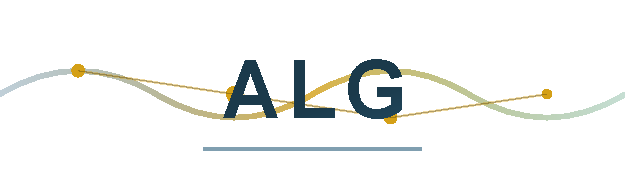
\includegraphics[width=\linewidth]{logo_ariel_symbol.pdf}
  \end{minipage}
\end{docentebox}

\medskip

% ── Soraya Corvalán ──────────────────────────────────────────
\begin{docentebox}[pescateal]{Soraya Corvalán — Ing. Pesquera · Gestión · Sostenibilidad · FAO}
  {\small\itshape\color{pescateal}
    Ingeniería Pesquera $|$ Gestión de Recursos Pesqueros $|$ Sostenibilidad $|$ FAO}\\[5pt]
  Primera mujer graduada como Ingeniera Pesquera en Argentina (UTN FRCh). Ingeniera
  pesquera con trayectoria destacada en investigación y gestión de recursos pesqueros
  y acuícolas. Investigadora en el INIDEP (2014--2020), donde desarrolló trabajos sobre
  dinámica de poblaciones, monitoreo de flotas y sostenibilidad. Consultora experta para la
  FAO en el proyecto TCP/ARG/4001D sobre fortalecimiento del sistema de información
  pesquera. Directora de la Red de Profesionales del Agro y Naturaleza (REDPAN).
  Consejera del programa \textit{Pampa Azul} (Ministerio de Ciencia, Tecnología e
  Innovación). Profesora Asociada Concursada en la UTN FRCh, Departamento de Ingeniería
  Pesquera. Coordinadora de la mesa redonda ``Industria 4.0 en el sector pesquero'' en
  el I CONIPE 2019. Colaboradora activa de la comunidad PesquerosEnIA.\\[7pt]
  \begin{tabular}{@{}ll}
    \textbf{LinkedIn:} & \href{https://www.linkedin.com/in/fishingengineer/}{linkedin.com/in/fishingengineer} \\
    \textbf{Empresa:}  & \href{https://www.linkedin.com/company/soraya-corvalan/}{linkedin.com/company/soraya-corvalan} \\
  \end{tabular}
\end{docentebox}

\medskip

% ── Damian Adolfo Giacone ─────────────────────────────────────
\begin{docentebox}[pescaocean]{Damian Adolfo Giacone — Lic. Sistemas · Máster Ind. 4.0 (IEBS) · IA · Ciberseguridad}
  {\small\itshape\color{pescaocean}
    Lic.\ en Sistemas y Computación $|$ Máster Industria 4.0 (IEBS) $|$ IA $|$ Ciberseguridad Industrial}\\[5pt]
  Licenciado en Sistemas y Computación (PUC Argentina) con Máster en Industria 4.0:
  Robótica, RPA, IoT e Inteligencia Artificial
  (\href{https://www.iebschool.com/}{IEBS School}, España). Más de 20 años de experiencia
  en tecnología aplicada al sector productivo. Lideró el área IT de Alpesca S.A.\ en
  Puerto Madryn (2003--2010), empresa líder del sector pesquero patagónico. Docente en
  UTN FRCh (2016--2022) y Docente Titular en la Universidad del Gran Rosario (UGR).
  Actualmente TCO en Legal-Hub y consultor independiente en automatización e IA para
  entornos industriales. Especialista en \textit{prompting} avanzado, diseño de agentes
  de IA y arquitecturas de datos para entornos productivos. Docente de PesquerosEnIA
  desde el I CONIPE 2019.\\[7pt]
  \begin{tabular}{@{}ll}
    \textbf{LinkedIn:} & \href{https://www.linkedin.com/in/damian-adolfo-giacone/}{linkedin.com/in/damian-adolfo-giacone} \\
    \textbf{IEBS:}     & \href{https://www.iebschool.com/}{iebschool.com} \\
  \end{tabular}
\end{docentebox}

\medskip

% ── Dr. Juan Domingo González (Docente Invitado) ─────────────
\begin{docentebox}[techgold]{Dr. Juan Domingo González — Docente Invitado · Acústica Computacional · IA · Estadística}
  {\small\itshape\color{techgold}
    Dr.\ Matemática Aplicada (UBA) $|$ Acústica Computacional $|$ IA $|$ Estadística Robusta $|$ SENASA}\\[5pt]
  Doctor en Matemática Aplicada (UBA, 2019), especializado en métodos de \textit{clustering}
  robusto y estadística computacional. Consultor en Inteligencia Artificial en el
  \textbf{SENASA} (Servicio Nacional de Sanidad y Calidad Agroalimentaria). Investigador
  asociado al DIIV-ARA/CONICET, donde desarrolla modelos computacionales de dispersión
  acústica para estimación de biomasa de anchoíta (\textit{Engraulis anchoita}) y otras
  especies pelágicas de la Plataforma Continental Argentina. Profesor en la
  \textbf{Universidad de Buenos Aires (UBA)} y en la \textbf{Universidad Nacional
  Guillermo Brown (UNGBrown)}. Autor de los paquetes de R publicados en CRAN:
  \texttt{RMBC} y \texttt{ktaucenters}, herramientas de clustering robusto con
  aplicaciones en análisis de datos oceanográficos y pesqueros.\\[7pt]
  \begin{tabular}{@{}ll}
    \textbf{CRAN -- RMBC:}         & \href{https://cran.r-project.org/package=RMBC}{cran.r-project.org/package=RMBC} \\
    \textbf{CRAN -- ktaucenters:}  & \href{https://cran.r-project.org/package=ktaucenters}{cran.r-project.org/package=ktaucenters} \\
    \textbf{LinkedIn:}             & \href{https://www.linkedin.com/in/juandgonzalez/}{linkedin.com/in/juandgonzalez} \\
  \end{tabular}
\end{docentebox}

\medskip
\noindent\textit{Docentes adicionales del programa (biografías en actualización):} \textbf{María Ana Reussi} y \textbf{Soledad Gurisich} (Unidad 1) · \textbf{Martín I.\ Errázquin} (Unidad 7).

% ═══════════════════════════════════════════════════════════════
%  10. BIBLIOGRAFÍA
% ═══════════════════════════════════════════════════════════════
\newpage
\printbibliography[title={Referencias Bibliográficas}]

\vfill
\begin{center}
  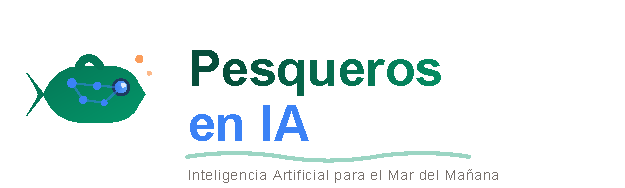
\includegraphics[height=1.0cm]{logo_pesqueros_full.pdf}\\[6pt]
  \small\color{stgray}
  \textit{Propuesta elaborada por el equipo docente PesquerosEnIA --- UTN FRCh, 2026.}\\
  Material de acceso abierto bajo licencia GPL-3.0.\\[3pt]
  {\color{pescateal}\url{https://github.com/PesquerosEnIA/curso-ia-produccion-pesquera}}
\end{center}

\end{document}
